% !TEX root=../../Thesis.tex
\newcommand {\matr}[2]{\left[\begin{array}{#1}#2\end{array}\right]}
\newcommand{\E}{\mathbb{E}}
\newcommand{\tr}{\mathrm{tr}}
\newcommand{\x}{{\mathbf{x}}}
\renewcommand{\u}{{\mathbf{u}}}
\newcommand{\w}{{\mathbf{w}}}
\renewcommand{\r}{{\mathbf{r}}}

\chapter{Modeling Intersection Driving Scenarios}
\label{ch:modeling_intersection}
% \begin{center}
%   \textit{\textbf{RQ 1: How can \gls{rl} be used to create a decision-making agent for driving through intersections?}}
% \end{center}
%   \vspace{12pt}

Navigating an intersection is a sequential decision-making problem that can be mathematically modeled using a \gls{mdp}, as introduced in Section~\ref{sec:background_mdp}. This thesis focuses on driving through intersections in the presence of other drivers, emphasizing not only to follow traffic rules but also the ability to adapt to the intentions of other drivers. Given that current sensors cannot directly observe other drivers' intentions, a \gls{pomdp} is a more suitable framework for formulating this problem.

% Driving through an intersection is a sequential decision-making problem and can be mathematically formulated using a \gls{mdp}, introduced in Section~\ref{sec:background_mdp}. As mentioned in the introduction, this thesis will focus on driving in intersections together with other drivers and not only follow the traffic rules but also be able to adapt to other drivers intentions. Since the intention of other drivers is not observable with any existing sensors today, \gls{pomdp} is better suited to formulate the problem. 

Effectively modeling the intersection problem is key for developing an optimal decision-making policy. This chapter will define the of the words intersection, intention and scenario used in this thesis. Although the some details in the \gls{pomdp} may differe between the papers, the general description is the same. Section \ref{sec:pomdp_fomulation} outlines the essential aspects of the \gls{pomdp} framework as applied to the intersection problem in this thesis.
 
% \Citet{Shalev2016} raises two concerns when using Machine learning, specially Reinforcement learning, for autonomous driving applications: ensuring functional safety of the Driving Policy and that the Markov Decision Process model is problematic, because of unpredictable behavior of other drivers.
% In the real world, intentions of other drivers are not always deterministic or predefined. Depending on their intention, different actions can be chosen to give the most comfortable and safe passage through an intersection.
% They also noted that in the context of autonomous driving, the dynamics of vehicles is Markovian but the behavior of other road users may not necessarily be Markovian.

% \section{Intersection scenarios}



% \begin{figure}
% \centering
% \begin{tikzpicture}
% 	\def\xstart{-7};

% 	% Crossing
% 	\draw[line width=0.5mm] (\xstart, 1) -- (-1, 1) -- (-1, 5);
% 	\draw[line width=0.5mm] (\xstart, -1) -- (-1, -1) -- (-1, -2);
% 	\draw[line width=0.5mm] (1, 5) -- (1, 1) -- (3, 1);
% 	\draw[line width=0.5mm] (1, -2) -- (1, -1) -- (3, -1);
	
% 	% cars
% 	\node[inner sep=0pt] (ego_car) at (-6,0)
% 	{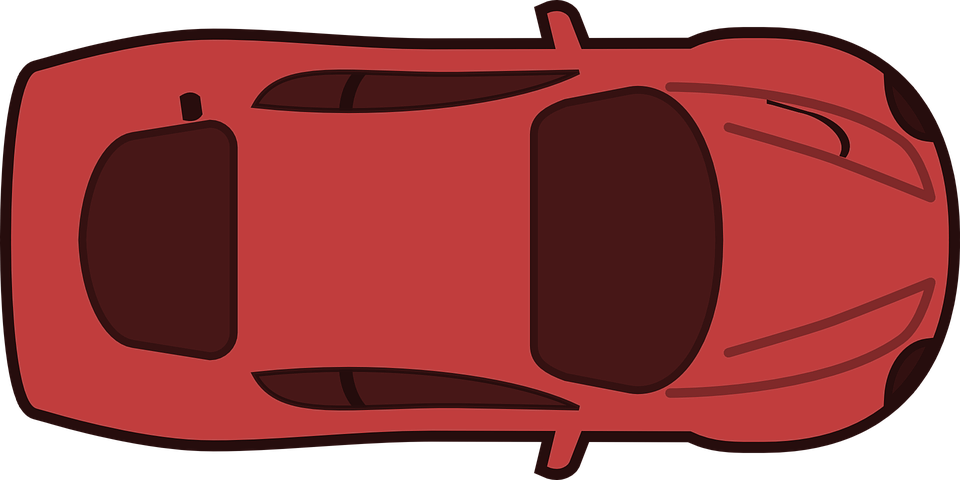
\includegraphics[width=.18\textwidth, angle=0]{figures/ego_car_top_down.png}};
% 	\node[inner sep=0pt] (target_car) at (0,4)
% 	{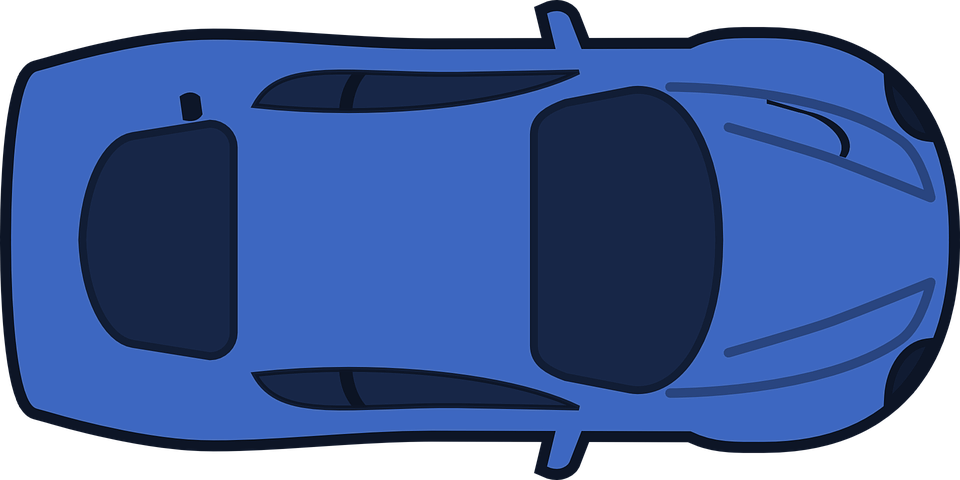
\includegraphics[width=.18\textwidth, angle=-90]{figures/target_car_top_down.png}};

% \end{tikzpicture}
% \caption{}
% \label{fig:intersection_scenario}
% \end{figure}


% Figure \ref{fig:intersection_scenario} shows a simple intersection with one crossing point. 
% \tommy{show examples of intersections.}
% \tommy{zone 0 - after intersection, zone 1 - conflict zone, zone 2 - right before the intersection, zone 3 - first obsereved interstion to zone 2}



\section{Intersections, intention and scenarios}
\label{sec:intro_intersections}
When it comes to the scenarios considered in this work. This section aims to clarify the use of the words' intersection, intention and scenario.
% When a pedestrian approach a crossing they have been taught at a young age to look at both sides of the road before crossing. The same apply for a human driver approaching an intersection. 
% When a human driver approach an intersection, it is natural to observe the environment to identify the traffic light, signs and other approaching vehicles. Then assess the situation, who has the right of way? 

% The intention of the other driver can be guided by the 
% Recently nontraditional intersections are also becoming increasingly popular. The goal of these designs is to reduce the number and/or severity of conflict points by altering the customary vehicular paths at the intersection. In light of the increased focus on and occurrence of these intersection types, it is expected that the application of nontraditional designs will continue to spread.

\begin{figure}[h]
	\centering
	\begin{subfigure}[t]{0.48\columnwidth}
		\centering
		\begin{tikzpicture}
			% Crossing
			\def\crossleftx{-2}
			\def\crossrightx{2}
			\def\crosstopy{2}
			\def\crossboty{-2}
			\def\roadwidth{0.5}

			\draw (0,0) circle (2pt);
			\node at (1.2, 0.2) {conflict point};
			\draw[thick] (\crossleftx, \roadwidth) -- (-\roadwidth, \roadwidth) -- (-\roadwidth, \crosstopy);
			\draw[thick] (\crossleftx, -\roadwidth) -- (-\roadwidth, -\roadwidth) -- (-\roadwidth-\roadwidth, \crossboty);
			\draw[thick] (\roadwidth, \crosstopy) -- (\roadwidth, \roadwidth) -- (\crossrightx, \roadwidth);
			\draw[thick] (\roadwidth-\roadwidth, \crossboty) -- (\roadwidth, -\roadwidth) -- (\crossrightx, -\roadwidth);

			% 	cars
			\node[inner sep=0pt] (ego_car) at (\crossleftx+0.5,0)
			{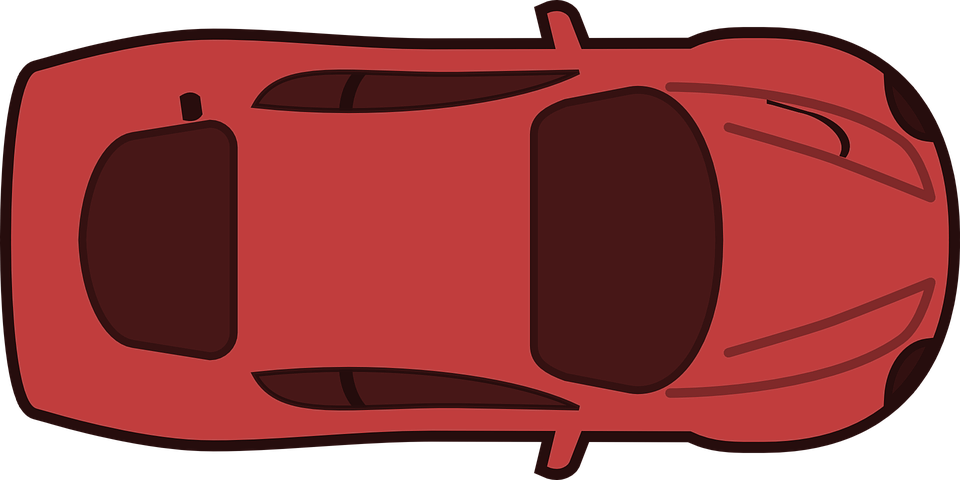
\includegraphics[width=.18\textwidth, angle=0]{figures/ego_car_top_down.png}};

			\node[inner sep=0pt] (target_car) at (0,\crosstopy-0.5)
			{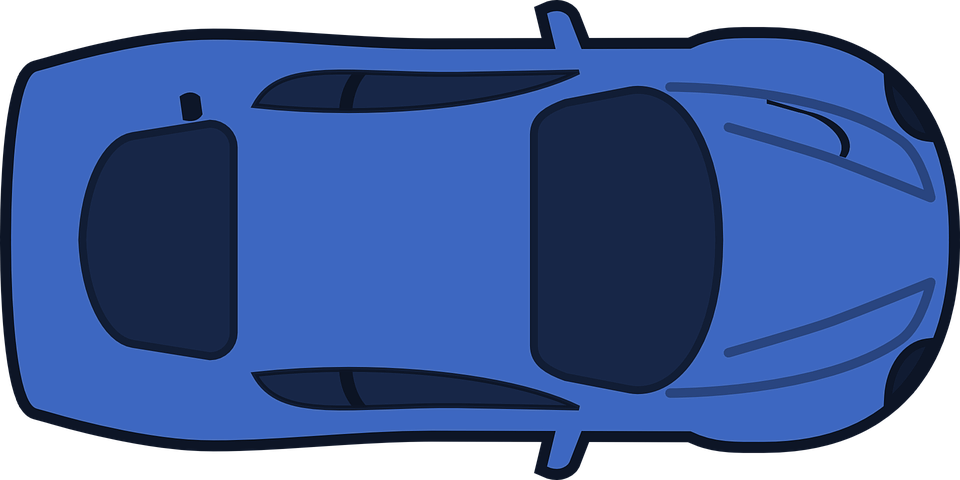
\includegraphics[width=.18\textwidth, angle=-90]{figures/target_car_top_down.png}};

			\node[inner sep=0pt] (target_car) at (-.1,-0.8)
			{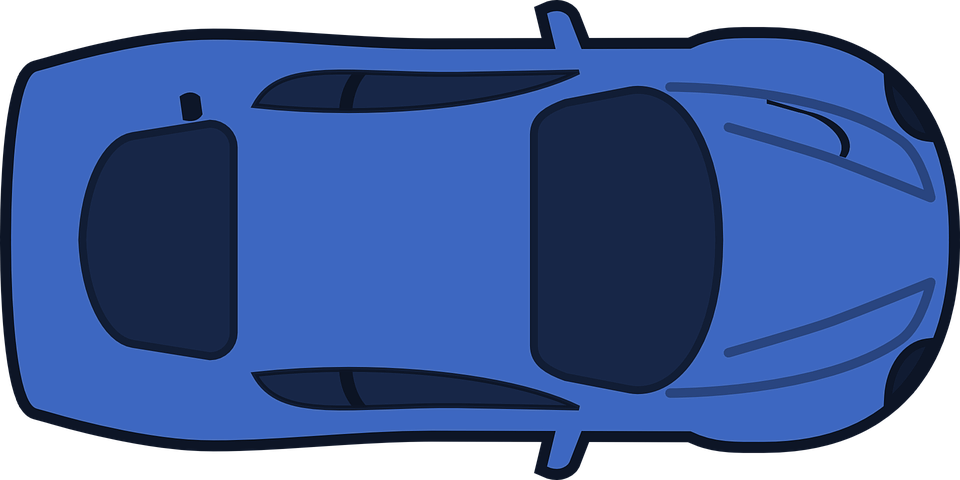
\includegraphics[width=.18\textwidth, angle=-110]{figures/target_car_top_down.png}};


		\end{tikzpicture}
		\caption{Single intersection}
\end{subfigure}%
	~ 
	\begin{subfigure}[t]{0.48\columnwidth}
		\centering
		\begin{tikzpicture}
			% Crossing
			\def\crossleftx{-2.5}
			\def\crossrightx{2.5}
			\def\crosstopy{2}
			\def\crossboty{-2}
			\def\roadwidth{0.5}

			\draw (-0.5,0) circle (2pt);
			\draw (0.5,0) circle (2pt);
			% \node at (0.7, 0.2) {crossing point$^1$};
			\draw[thick] (\crossleftx, \roadwidth) -- (-\roadwidth-0.5, \roadwidth) -- (-\roadwidth-0.5, \crosstopy);
			\draw[thick] (\crossleftx, -\roadwidth) -- (-\roadwidth-0.5, -\roadwidth) -- (-\roadwidth-0.5, \crossboty);
			\draw[thick] (0, \crosstopy) -- (0, \roadwidth);
			\draw[thick] (0, -\roadwidth) -- (0, \crossboty);
			\draw[thick] (\roadwidth+0.5, \crosstopy) -- (\roadwidth+0.5, \roadwidth) -- (\crossrightx, \roadwidth);
			\draw[thick] (\roadwidth+0.5, \crossboty) -- (\roadwidth+0.5, -\roadwidth) -- (\crossrightx, -\roadwidth);

			% 	cars
			\node[inner sep=0pt] (ego_car) at (\crossleftx+0.5,0)
			{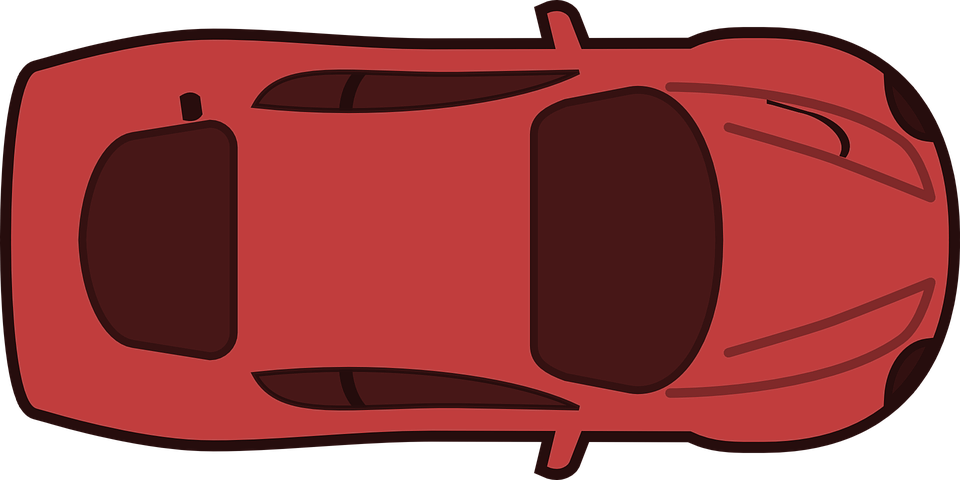
\includegraphics[width=.18\textwidth, angle=0]{figures/ego_car_top_down.png}};

			\node[inner sep=0pt] (target_car) at (-0.5,\crosstopy-0.5) {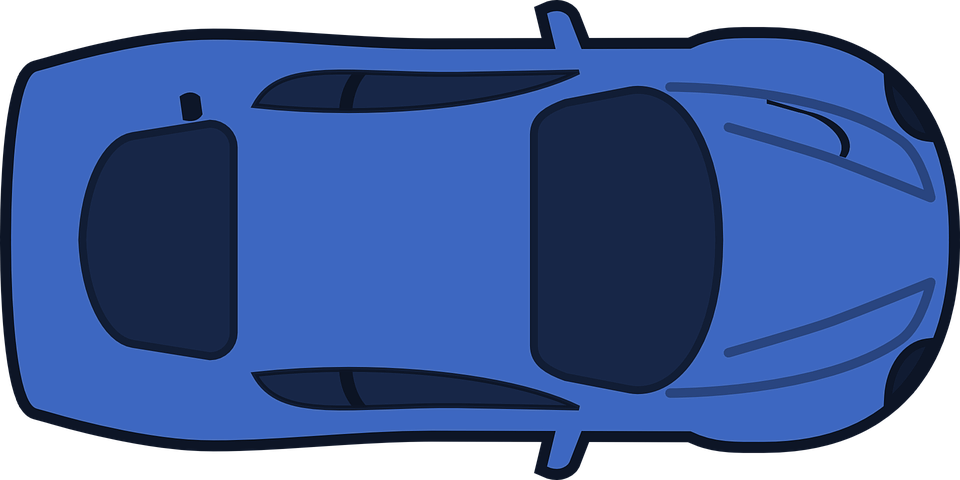
\includegraphics[width=.18\textwidth, angle=-90]{figures/target_car_top_down.png}};

			\node[inner sep=0pt] (target_car_2) at (0.5,\crossboty+0.5) {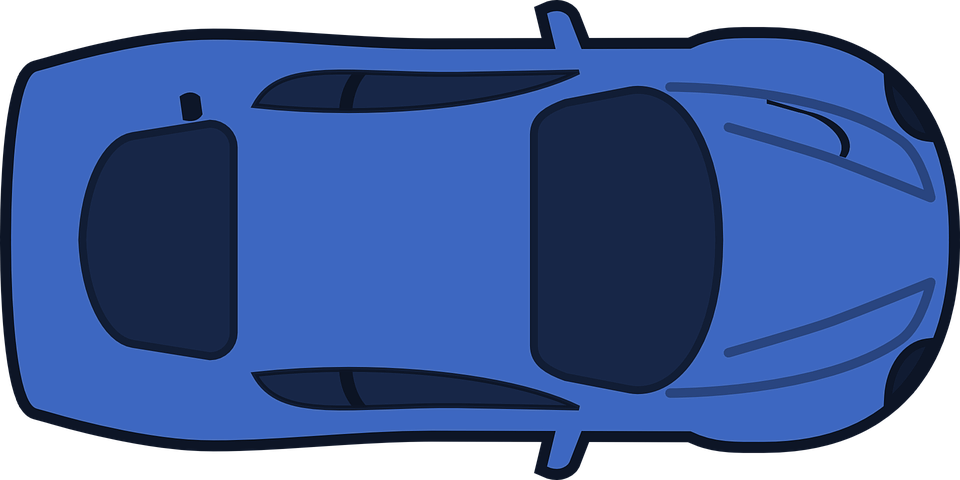
\includegraphics[width=.18\textwidth, angle=90]{figures/target_car_top_down.png}};

		\end{tikzpicture}
		\caption{Double intersection}
	\end{subfigure}

	\caption{Examples of different intersections}
	\label{fig:example_intersections}
\end{figure}
Let's begin by defining the terms 'intersection,' 'intention,' and 'scenario' within the context of this study.
An intersection refers to the geometric layout of roads intersecting each other, encompassing elements such as the number of junctions, conflict points, turns, and angles of incidence, as illustrated in Figure~\ref{fig:example_intersections}. 
Intersections can be categorized as signalized or unsignalized. A signalized intersection is equipped with mechanisms to designate the right-of-way, such as regulatory signs (e.g., STOP or YIELD) or traffic signals, while an unsignalized intersection lacks such features. However, as emphasized in the introduction, human drivers do not always adhere strictly to these right-of-way rules, which can result in accidents. Therefore, this thesis defines intentions as the anticipated actions of other vehicles in the future, such as stopping, cautiously slowing down, or proceeding through the intersection.

\begin{figure}[h]
	% \mbox{\parbox{\textwidth}{
	% \centering
	% % \vspace{0.3cm}
	% 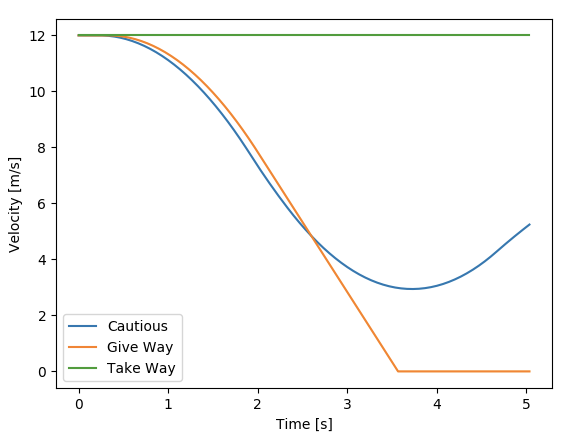
\includegraphics[width=0.6\columnwidth]{YourThesis/papers/mpc/figures/velocity_profiles_agents.png}
	% }}
	\centering
	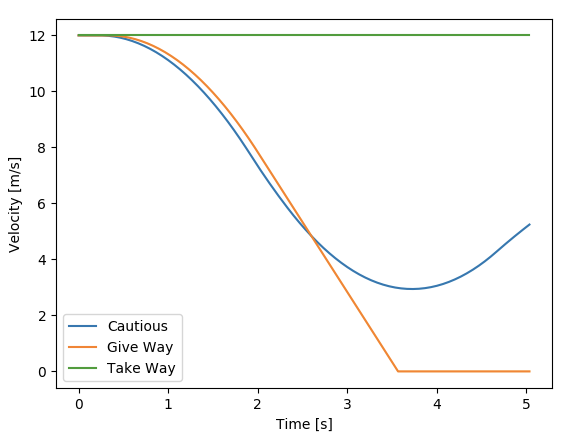
\includegraphics[width=0.6\columnwidth]{YourThesis/papers/mpc/figures/velocity_profiles_agents.png}

	\caption{An illustration showing velocity profiles for agents with three distinct intentions. Each agent shares the same initial position and velocity while approaching a common intersection.}
	\label{fig:intro_intention_profiles}
	% \vspace{-0.3cm}
\end{figure}

Figure \ref{fig:intro_intention_profiles} illustrates how velocity profiles can differ for three different intentions. In this example, distinguishing between the 'give way' and 'take way' intentions is straightforward, as the velocity begins to decelerate at time $0$. However, identifying the 'cautious' intention poses a challenge, as the agent cannot be certain until the other vehicle comes to a complete stop.

If intentions are known, intersections can be treated as unsignalized, as the right-of-way can be inferred from the intentions rather than relying solely on infrastructure. This approach ensures safety even in situations where another vehicle disregards traffic rules, such as running a red light, as a cautious agent will prioritize safety and stop accordingly.

\section{The intersection problem}
\begin{figure}
	\mbox{\parbox{\textwidth}{
		\centering
		\begin{tikzpicture}
			\def\xstart{-7};

			\coordinate (p) at (3,0);
			\foreach \n/\w/\c in {z0/2/green,z1/2/red,z2/2.5/orange,z3/3.5/blue}{
				\node[rectangle,
				draw=none,
				anchor=east,
				text = black,
				fill = \c!60,
				minimum width = \w cm, 
				minimum height = 2cm] 
				(n) at (p) {\Huge \n};
				
				\coordinate (p) at (n.west);
			}

			% Crossing
			\draw[line width=0.5mm] (\xstart, 1) -- (-1, 1) -- (-1, 5);
			\draw[line width=0.5mm] (\xstart, -1) -- (-1, -1) -- (-1, -2);
			\draw[line width=0.5mm] (1, 5) -- (1, 1) -- (3, 1);
			\draw[line width=0.5mm] (1, -2) -- (1, -1) -- (3, -1);
			
			% cars
			\node[inner sep=0pt] (ego_car) at (-7,0)
			{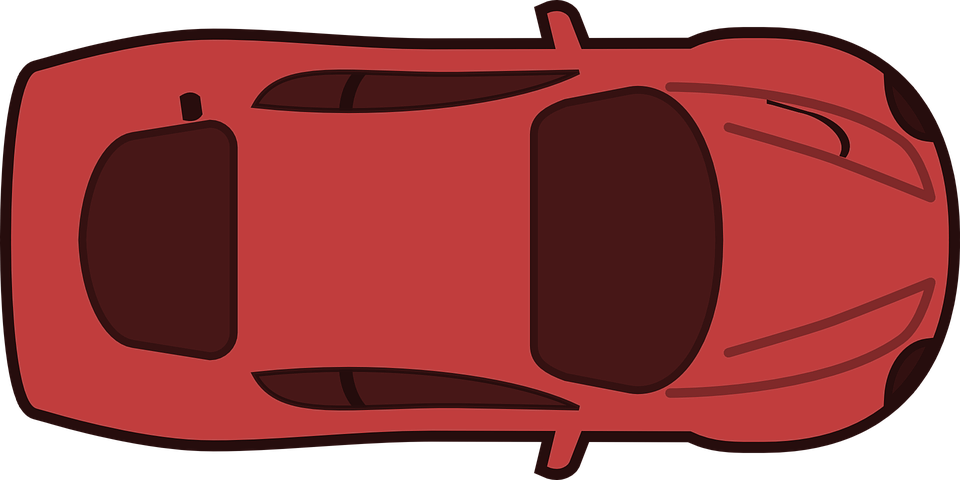
\includegraphics[width=.18\textwidth, angle=0]{figures/ego_car_top_down.png}};
			\node[inner sep=0pt] (target_car) at (0,4)
			{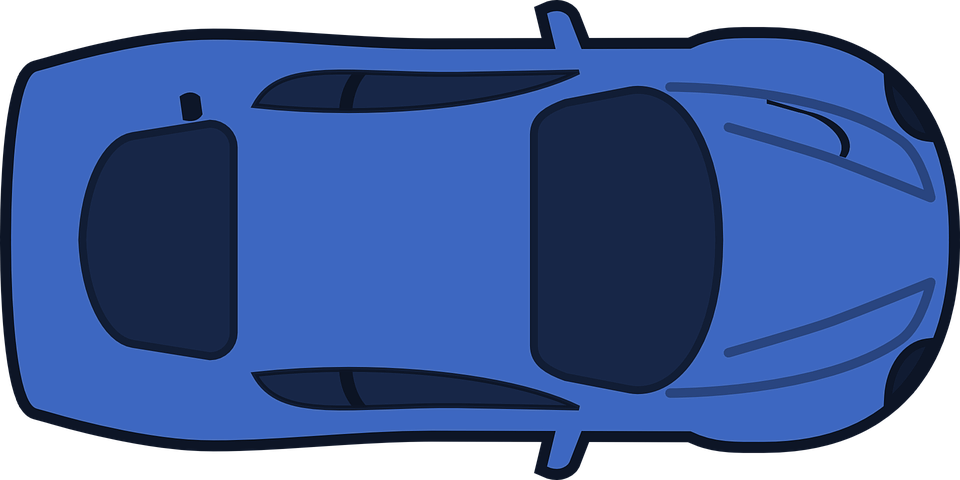
\includegraphics[width=.18\textwidth, angle=-90]{figures/target_car_top_down.png}};

	\end{tikzpicture}
	}}
	\caption{Intersection scenario divided into zones describing what is required of the decision maker in different zones}
	\label{fig:zones}
\end{figure}

With the \gls{mdp} defined, the path of the ego vehicle can be segmented into four zones as shown in Figure~\ref{fig:zones}. Starting from the end, Zone 0 represents the 'safe zone,' where the ego vehicle is out of danger and can resume nominal driving. Zone 1 is the 'conflict zone,' where a collision with another vehicle is possible. Zone 2, the 'critical decision zone,' is the final opportunity for the vehicle to either stop or proceed through the intersection. The size of zone 2 is determined by the minimum distance required for the vehicle to come to a complete stop before entering the conflict zone, ensuring sufficient time for safe decision-making. Lastly, Zone 3, the 'information gathering zone,' is situated furthest from the intersection. Here, the agent can observe how other vehicles behave over time to estimate their intentions.

The goal is to reach Zone 0. To achieve this, the agent aims to minimize the time spent in Zone 1 if there is a chance of intersection with another car. Our actions are formulated as short-term goals, designed for comfortable use with lower acceleration rates. The size of Zone 2 depends on the vehicle's current speed, which is influenced by its behavior in Zone 3.

Now, two conflicting strategies emerge: to minimize time in Zone 1, the agent desires a high speed entering the intersection. However, it also seeks a low speed to reduce the size of Zone 2 and the critical decision period. If the intentions of other vehicles are known, the stochasticity in Zone 1 would be eliminated, transforming the problem into a scheduling task aimed at creating a velocity profile that minimizes the time required to cross. However, since the intentions of other vehicles are stochastic, reinforcement learning offers a promising approach to address this uncertainty and optimize decision-making in dynamic traffic scenarios.

\section{\gls{pomdp} formulation}
\label{sec:pomdp_fomulation}
\subsection{State space}
\begin{figure}[h]
	\centering
	\begin{tikzpicture}
	
		% Crossing
		\def\crosstopy{5}
		\def\crossboty{-2.5}
		\def\crossleftx{-5}
		
		\draw[thick] (\crossleftx, 1) -- (-1, 1) -- (-1, \crosstopy);
		\draw[thick] (\crossleftx, -1) -- (-1, -1) -- (-1, \crossboty);
		\draw[thick] (1, \crosstopy) -- (1, 1) -- (3, 1);
		\draw[thick] (1, \crossboty) -- (1, -1) -- (3, -1);
		
		cars
		\node[inner sep=0pt] (ego_car) at (-4,0)
		{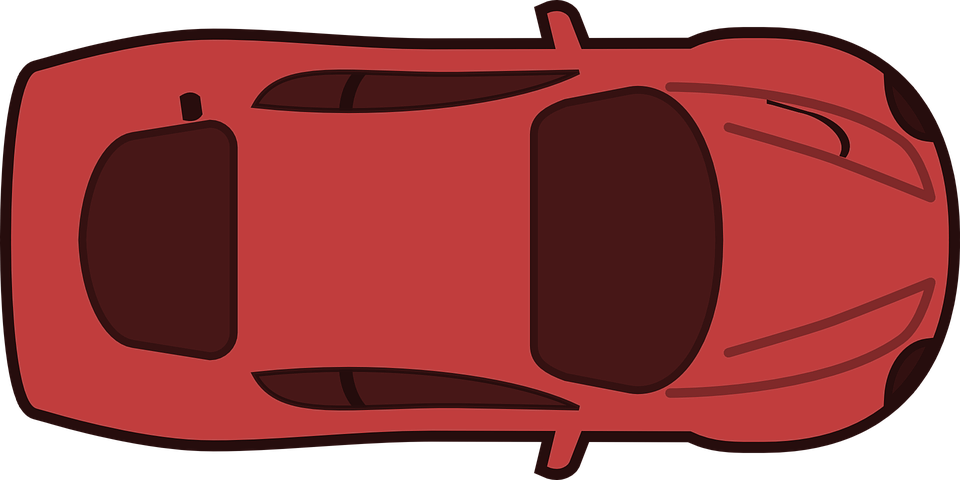
\includegraphics[width=.18\textwidth, angle=0]{figures/ego_car_top_down.png}};
		\draw[->] ([yshift=0.2cm]ego_car.east) -- node[above] {$p_\mathrm{ego}, v_\mathrm{ego}$} ($ (ego_car) + (2.5,0.2)$ );
		% \draw[|-|] ([yshift=-0.2cm]ego_car.east) -- node[below] {$p_{ego}$} (-1,-0.2);
	
		% \node[inner sep=0pt] (target_car_3) at (0,7)
		% {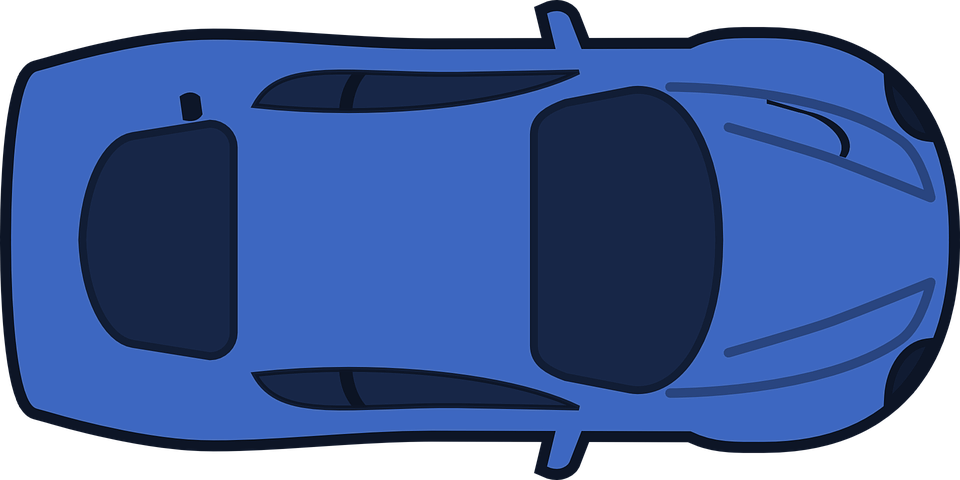
\includegraphics[width=.18\textwidth, angle=-90]{figures/target_car_top_down.png}};
		% \node (tc_text3a) [right=of target_car_3, align=center] {Car $n$};
		% % \node (tc_text3b) [left=of target_car_3, align=center] {Conflict Car};
		% \draw[->] ([xshift=-.3cm]target_car_3.south) -- node[right] {$p_{n} v_{n} \zeta_n$} ($ (target_car_3) + (-.3,-2)$ );
		% \draw[|-|] ([xshift=-0.8cm]target_car_3.south) -- (-.8,1);
		% \node (tc_tti) [below left= 0.9cm and -0.7cm of target_car_3, align=center] {$p_n$  \\ $\tau_{int}$};
	
		\node[inner sep=0pt] (target_car_2) at (0,3.5)
		{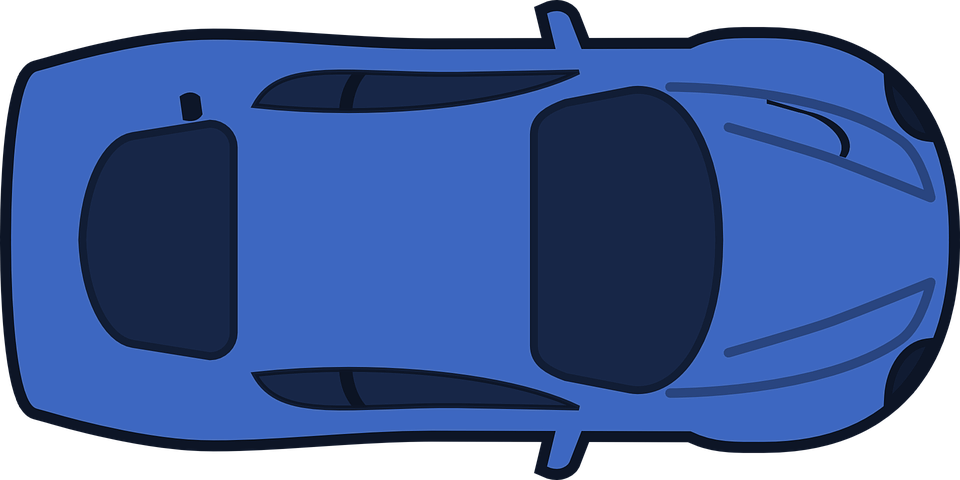
\includegraphics[width=.18\textwidth, angle=-90]{figures/target_car_top_down.png}};
		\node (tc_text2) [right=of target_car_2] {Car $n$};
		\draw[->] ([xshift=-.3cm]target_car_2.south) -- node[right] {$p_{n} v_{n} \zeta_n$} ($ (target_car_2) + (-.3,-2)$ );
		
		\node[inner sep=0pt] (target_car_1) at (0,-1.5)
		{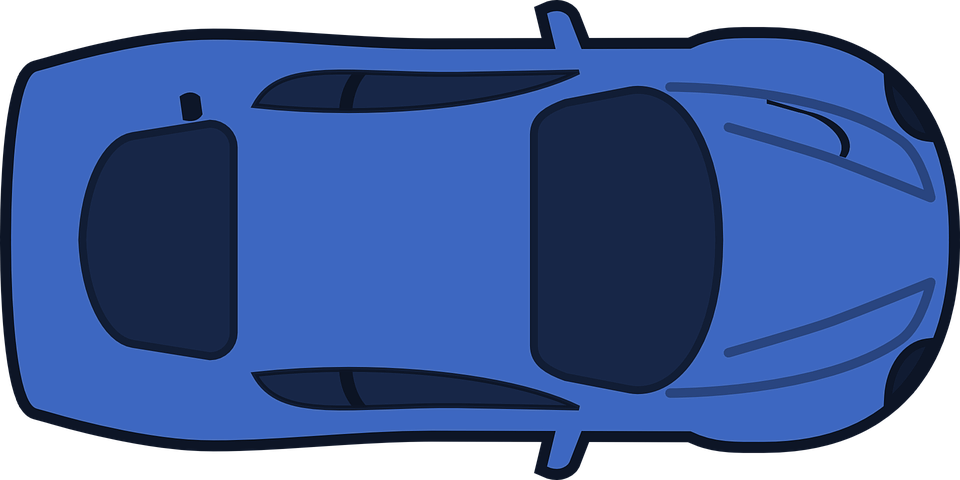
\includegraphics[width=.18\textwidth, angle=-90]{figures/target_car_top_down.png}};
		\node (tc_text1) [right=of target_car_1] {Car 1};
	
	\end{tikzpicture}
	\caption{General description of the states in a simple intersection. The ego vehicle in red is controlled by the agent, while the blue vehicles are the other vehicles crossing the same intersection. Each blue vehicle is described by an index $n$, a position $p_n$, a velocity $v_n$  and hidden intention $\zeta_n$}.
	\label{fig:intersection_scenario}
	\end{figure}

From Section~\ref{sec:background_mdp}, the state space contains all the information necessary about the agent and environment to be able to transition to any given state. In the scenario shown in Figure~\ref{fig:intersection_scenario}, the red car on the horizontal lane represents the ego vehicle controlled by the agent while the blue cars on the vertical lane are the other vehicles which ego needs to interact with in order to cross the intersection. 

% Let's start by defining the information needed. 
Instead of using a Cartesian coordinate system to describe the postiion $p_\mathrm{ego}$ and $p_n$, relative distance measures are proposed instead. This way, states describing the intersection and its participants are generalizable to different intersection designs, e.g., the angle of incidence and number of crossing points. 

The velocity of ego $v_\mathrm{ego}$ and all other the traffic participants $v_n$ is necessary to be able to predict what position they will be in the next state. Finally, the intention of all the other participants $\zeta_n$. As mentioned in Section \ref{sec:intro_intersections}, $\zeta_n$ encapsules information such as stop sign, traffic light or even inattention in to one state. 
\paperBelief shows a comparison between two fully observable \gls{mdp}s, one with intention and the other one without and the results show that having an intention state reduce number of collisions. 
\paperLSTM used a \gls{lstm} network architecture to implicitly predict $\zeta$. %The states describing ego and other vehicle are spearated. Repeat the states for each other vehicle we observe. 
\todo{add results for with and without $\zeta$ and DRQN and DQN}

\subsection{Action space}
\tommy{options, take way, give way, follow car}
One of the limitations of deep Q-learning is that the action space has to be discreet. In other work it is common to set the action space to different acceleration request\cite{bouton2019}. \paperLSTM proposed using short-term goals as actions. The short term goals are high level objectives like stop at the start of the intersection, follow car with id $n$ or drive through the intersection following a reference speed. This high level action is then converted to a set pf parameters sent to a sliding mode controller that generates an acceleration, which controls the ego car. 
% The sliding mode implementation in \paperLSTM could only follow one car at a time and relied on the Q-learning algorithm to switch between actions and control the velocity. 
While in \paperMPC the actions in instead sent to a \gls{mpc} to generate a velocity profile. The \gls{mpc} could take consecutive intersection points into account and create a velocity profile for a short time horizon, where the action would instead be which gap between cars to drive through.

\gls{mpc} is good at creating a plan within some given constraints but has a mixed integer problem and calculating the optimal path for all possible action is very computationally heavy. While Q-learning is good at estimating the value of an action given a state, but needs to explore many bad actions before converging to a good one. Combining \gls{rl} and \gls{mpc} enabled an agent efficiently choose a good action that the \gls{mpc} could use to create a safe and efficient velocity profile for. 

\subsection{Transistion model}
The transition model is not known and \gls{rl} is used to learn this model by taking actions in the environment from different states and recording the reward and what state the agent transition into.
The environment in this work is a simulator and the main thing the agent is trying to learn is the transition of the other vehicles which depends on their intentions $\zeta$. 
The intentions are models as predetermined actions while folloing a \gls{idm} ontop of that. This makes the interaction between cars more complicated. 
\tommy{IDM, and other agents behaviors/intentions.}
\paperLSTM random parameters, speeds and spawn rates. 
\paperMPC cautious, give way, take way


\subsection{Observation model}
The observation model can be interpreted as the noise from the sensors, \paperLSTM assumes perfect sensing while \paperBelief has some added noise to the observed states. 
The observation space is usually the same as the state space without the intention state $\zeta$. Because there are no sensors that can detect other drivers intentions. 
\tommy{Everything in the state space except intention. Everything that is observable through the sensors in the car. }

\subsection{Reward function}
The design of the reward function is what determine the value of each state. A well crafted reward function will lead to a good driving policy. 
Designing the reward model from the objective the agent are trying to achieve. Starting of a relative reward difference around 0 and 1. Then hand tune to get a performance close to the desired outcome. 
All papers formulated the reward based on the terminal states: goal, collision and timeout. 
\paperLSTM and \paperMPC has a continious negative reward for change in acceleration to punish jerk that would come from changing between actions that would make it uncomfortable for the passengers. 
\paperLSTM also gives a relative large negative reward for choosing to follow a car that does not exist. 

\tommy{The reward function takes in the predicted outcome of the model in the MPC and can penalize the choice of action. but if experience show that the outcome is better than the model, it can choose to take a bad action that would lead to a better total reward compared to only following a conservative model. }

\section{Results from simulation}

% \begin{figure}[t!]
	% \mbox{\parbox{\textwidth}{
% 	\centering
% 	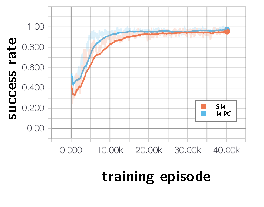
\includegraphics[width=\columnwidth]{YourThesis/papers/mpc/figures/figures-successrate.pdf}
% }}
% 	\caption{Average MPC and SM success rate for a single corssing after evaluating the policy 300 episodes.}
% 	\label{fig:result1}
% \end{figure}

% \begin{figure}[t!]
% 	\centering
% 	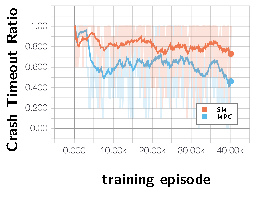
\includegraphics[width=\columnwidth]{YourThesis/papers/mpc/figures/figures-crashratio.pdf}
% 	\vspace{-4em}
% 	\caption{Average MPC and SM crash to timeout ratio for a single crossing after evaluating the policy in 300 episodes. A CTR of $0$ means that all failures are timeouts, while a CTR of $1$ means that all failures are collisions.}
% 	\label{fig:result2}
% \end{figure}

\begin{table}[h]
	\mbox{\parbox{\textwidth}{
	\centering
	\begin{tabular}{ |p{1,6cm}||p{1,2cm}|p{1,2cm}|p{1,2cm}|p{1,2cm}|}
	\hline
	Controller &\multicolumn{2}{|c|}{Success Rate}
	&\multicolumn{2}{|c|}{Timeout Ratio}\\
	\hline
	 & Single & Double & Single & Double\\
	\hline
	SM & $96.1\%$ & $90.9\%$ & $72\%$ & $93\%$\\
	MPC & $97.3\%$ & $95.2\%$ & $45\%$ & $76\%$\\
	\hline
	\end{tabular}
	}}
	\caption{Average success rates and collision to timeout rates.}% across single and double crossings.}   

% \label{tab:successrate}
\end{table}

synergies between mpc and dqn


\section{Discussion}
Why is it hard. 
\tommy{zone 0 - after intersection, zone 1 - conflict zone, zone 2 - right before the intersection, zone 3 - first obsereved interstion to zone 2}

\begin{figure}
	\mbox{\parbox{\textwidth}{
		\centering
		\begin{tikzpicture}
			\def\xstart{-7};

			\coordinate (p) at (3,0);
			\foreach \n/\w/\c in {z0/2/green,z1/2/red,z2/2.5/orange,z3/3.5/blue}{
				\node[rectangle,
				draw=none,
				anchor=east,
				text = black,
				fill = \c!60,
				minimum width = \w cm, 
				minimum height = 2cm] 
				(n) at (p) {\Huge \n};
				
				\coordinate (p) at (n.west);
			}

			% Crossing
			\draw[line width=0.5mm] (\xstart, 1) -- (-1, 1) -- (-1, 5);
			\draw[line width=0.5mm] (\xstart, -1) -- (-1, -1) -- (-1, -2);
			\draw[line width=0.5mm] (1, 5) -- (1, 1) -- (3, 1);
			\draw[line width=0.5mm] (1, -2) -- (1, -1) -- (3, -1);
			
			% cars
			\node[inner sep=0pt] (ego_car) at (-7,0)
			{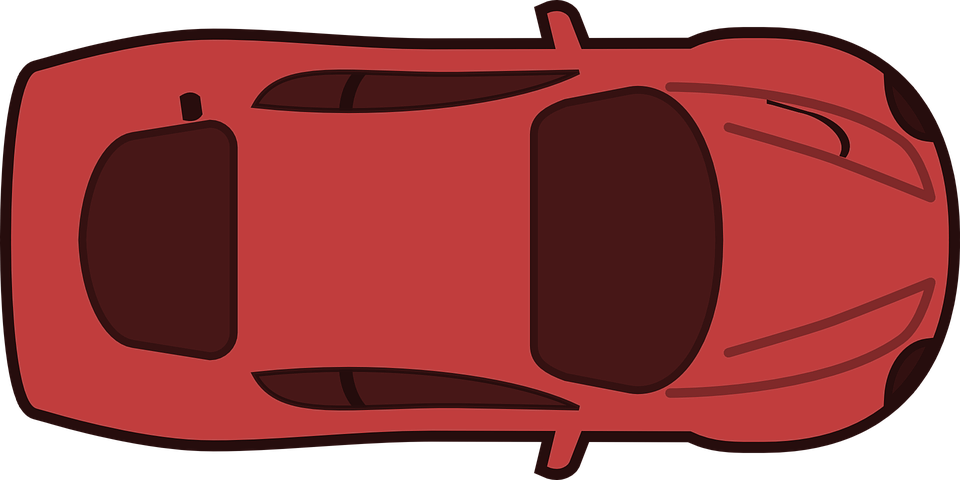
\includegraphics[width=.18\textwidth, angle=0]{figures/ego_car_top_down.png}};
			\node[inner sep=0pt] (target_car) at (0,4)
			{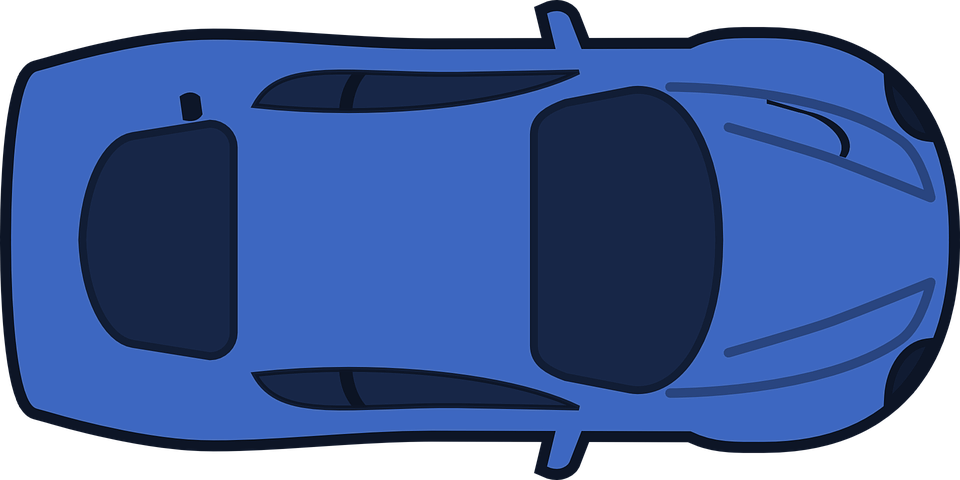
\includegraphics[width=.18\textwidth, angle=-90]{figures/target_car_top_down.png}};

	\end{tikzpicture}
	}}
	\caption{Intersection scenario divided into zones describing what is required of the decision maker in different zones}
	\label{fig:zones}
\end{figure}

With the \gls{mdp}, defined a typical intersection can be described as in Figure \ref{fig:zones}. From the figure the path of the ego vehicle can be divided into four zones. Starting from the end, zone 0 is the "safe zone" where the ego is our of danger and can return to nominal driving. Zone 1 is the conflict zone, this is where there is a possibility to collide with another vehicle. Zone 2 is critical decision zone, where this is the last chance the vehicle has to stop or cross. The size of this zone is defined as the minimal distance the car needs to come to a complete stop to the start of the conflict zone. The final zone is zone 3, the information gathering zone, and is the furthest from the intersection and where the agent can observe the scenario and the other vehicles behavior over time. 

the goal is to reach zone 0, 
to do this the agent would want to minimize the time in zone 1, if there is chance of intersection with another car.
Because our actions are formulated as options and designed to be conformtable with lower acceleration rates. The size of zone 2 is dependent on the vehicels current speed, which is dependent on how the vehicle behaved in zone 3. 
Now there are two conflicting strategies, to minimize time in zone 1 the agent wants a high speed coming into the intersection. while it would want a low speed to shorten the zone 2 and the critical decision. 

If the intention of the other vehicles is known the stochasticity in zone 1 would be gone and the problem becomes a scheduling problem of creating a velocity profile that minimizes the time to cross.  

\tommy{Deep Q-learning approach}
We want to formulate the problem in such a way that abstracts the information of traffic lights, traffic signs and intention. This way the car is closer to L5 by not relying on the different traffic lights.

One motivation example is in how traffic lights works. In Sweden, we have sensors that can sense if there are cars in an intersection and create a traffic light schedule accordingly, compared to the US where the traffic signals set up using timers. As a consequence, Drivers approaching a yellow light 

The \gls{dqn} algorithm uses a \gls{nn} and has two disadvantages. One is that the size of the network is fixed, this forces the input space to be fixed. Our state space is defined by the physical state of the surrounding cars, and the number of cars we observe at each situation variate. %Therefor we need a way to invariate of 

% \section{Approach (State representation, observable and unobservable)}
% This paper explored the possibility of solving the problem with \gls{rl} by trying a verity of different methods from the rainbow paper with the addition to the LSTM layer and presented the results that had the highest impact on the conversion. 
% \todo{State representation}
% This section describes the general state representation used in this research that enables these methods to be generalizable for different type of intersection and crossings. 
% By describing the state space as a set of distances to intersection points, we can abstract the map layout of different intersections and the same algorithms would work for intersections variations that we haven't specifically trained on. 
% \todo{add image of intersection scenario with 90 degree entry point and 45 degree entry point.}
% \todo{Network model}
% Shared weights, DQN vs DRQN. 
% \todo{Learning tools}
% experience replay and dropout. 
% \todo{explain rewards}
% large negative reward for invalid actions.
% \section{Simulated experiments}
% \section{Results and discussion}
% \begin{itemize}
%   \item STG as actions
%   \item shared weights
%   \item effect of replay, dropout 
%   \item comparing a dqn and Drqn 
% \end{itemize}
% however sensitive to noise. 

% LSTM take into account the history, but when applied in the real world with noise the model did not perform as well. 
% The immidiate reward for jerk is 
% \tommy{finding time to intersection and position itself in a way that does not conflict with other cars.}

% \tommy{FIND A SECTION. Collisions in this thesis, may sound critical and extreme. But collisions in this content is for the purpose of the simulator and for the terminal state of the agent. Translated to a system perspective, it would mean that a backup collision avoidance algorithm had to interfere and in the worst case take over. }

 

